% ----------------------------------------------------------
% Fundamentação Teórica
% ----------------------------------------------------------
\chapter{Fundamentação Teórica}

\section{Crowdsourcing}
% Definição
Antes de se falar de Crowdfunding é importante conhecer o movimento o qual originou. Crowdsourcing foi definido por \citeauthor{wired-crowdsource} em \citeyear{wired-crowdsource} como o ato de uma companhia ou instituição pegar uma função desempenhada por seus funcionários e terceiriza-la para uma rede anônima geralmente bastante grande de pessoas na forma de uma chamada aberta. Isso pode tomar a forma de um sistema cooperativo, onde o trabalho é feito de forma colaborativa, mas também frequentemente o trabalho é executado por indivíduos. O prerrequisito crucial é o uso de um formato de chamada aberta e a grande rede de potenciais trabalhadores para atendê-lo.

% Exemplos
Essa modalidade de terceirização não é recente. Por exemplo em 1714 o Governo Britânico conduziu um concurso chamado Prêmio Longitude\cite{wiki-longitude_rewards}, que daria como recompensa 10 a 20 mil libras, dependendo da qualidade da solução, para quem resolvesse um dos maiores problemas da época: como determinar a longitude de uma embarcação em alto-mar.

Um segundo exemplo notável é o de \citeauthor{hearn2002tracks} que conta como Matthew Fontaine Maury, em 1848, distribuiu de forma gratuita 5000 cópias de seu catálogo de correntes marítimas e eólicas pedindo em troca que os marinheiros fizessem e entregassem seus diários de bordo ao retornar de suas jornadas.

Com avanços nas técnicas de desenvolvimento de software, computação distribuída, processamento de dados e a popularização da Internet a partir da década de 1990 projetos como o \emph{Great Internet Mersenne Prime Search}\footnote{Projeto para buscar Primos de Mersenne (números resultantes de \( 2^p - 1 \)) - http://www.mersenne.org} (GIMPS), lançado em 1996, e o SETI@Home\footnote{Análise de ondas de rádio cósmicas em busca de vida extra terrestre - https://setiathome.berkeley.edu}, lançado em 1999, começaram a utilizar do poder de processamento latente nos computadores pessoais de inúmeros voluntários ao redor do planeta para executarem tarefas massivas que, sem isso, necessitariam de supercomputadores e bastante investimento.

Naturalmente esse aspecto da coletivização da ajuda evoluiu para além da realização de tarefas, grandes ou pequenas, e surgiram novas modalidades de Crowdsourcing, a mais prominente sendo o Crowdfunding.



\section{Crowdfunding}
Falar de crowdfunding de forma técnica.



\section{Empreendedorismo Social}
Falar de crowdfunding de forma técnica.

\begin{figure}[H]
  \centering
  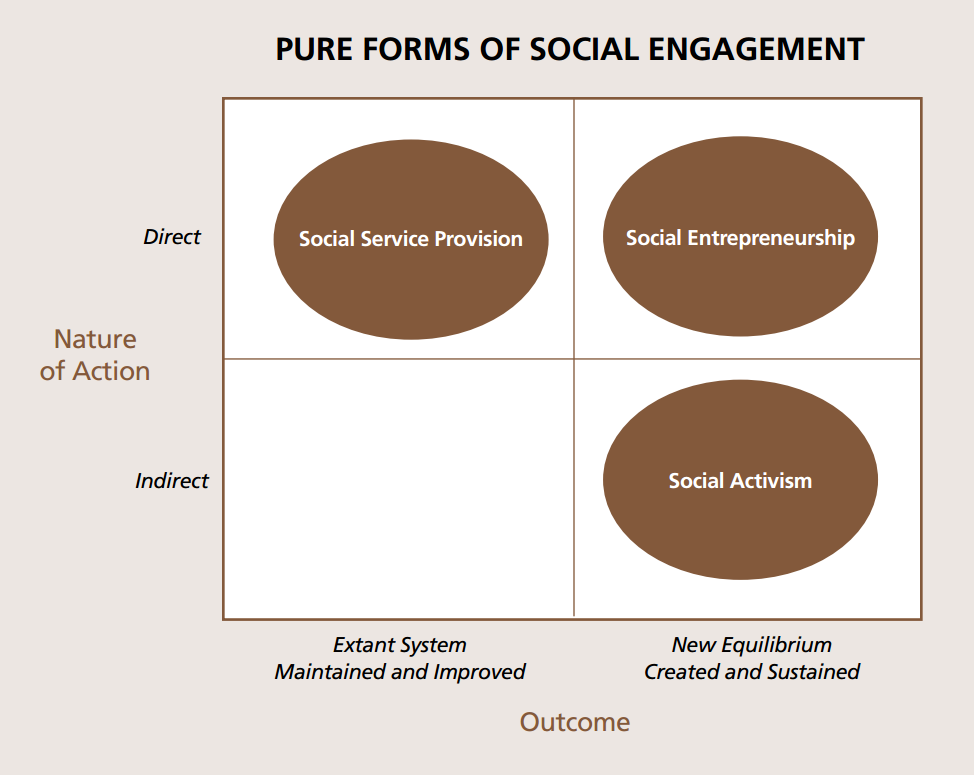
\includegraphics[scale=0.4]{imagens/formas-engajamento-social}
  \caption{Formas de Engajamento Social}
  \label{Rótulo da Imagem}
\end{figure}

Coloquei uma imagem aqui pois provavelmente vou utilizá-la.

E uma tabela, só para ter uma:

\begin{table}[]
\centering
\begin{tabular}{lll}
\multicolumn{1}{c}{\textbf{They Claim To Value}}   & \multicolumn{1}{c}{\textbf{They Really Value}}             & \multicolumn{1}{c}{\textbf{We Fucking Do}}     \\ \hline
\multicolumn{1}{|l|}{Individuals and interactions} & \multicolumn{1}{l|}{Tons of billable hours}                & \multicolumn{1}{l|}{Programming, Motherfucker} \\ \hline
\multicolumn{1}{|l|}{Working software}             & \multicolumn{1}{l|}{Tons of pointless tests}               & \multicolumn{1}{l|}{Programming, Motherfucker} \\ \hline
\multicolumn{1}{|l|}{Customer collaboration}       & \multicolumn{1}{l|}{Bleeding clients dry}                  & \multicolumn{1}{l|}{Programming, Motherfucker} \\ \hline
\multicolumn{1}{|l|}{Responding to change}         & \multicolumn{1}{l|}{Instability and plausible deniability} & \multicolumn{1}{l|}{Programming, Motherfucker} \\ \hline
\end{tabular}
\caption{Besteira do Programming-Motherfucker}
\label{label-da-tabela}
\end{table}



\section*{Resumo}
Aqui falamos de blablabla e de xpto.